\documentclass[main.tex]{subfiles}
\section{2 point Boundary Value Problems}
2-point Boundary Value Problems (BVP) represent a special case of differential equations where the solution is limited by a pair of constraints at both ends of the interval. Hence, the task consists of finding the solution that apart from solving the differential equation satisfies the boundary conditions.

In the linear case, a numerical approximation to the  solution to these problems can be obtained solving a linear system. However, for nonlinear differential equations the solution is not straightforward and an iterative process is needed. In this exercise, we shall study different methods for solving nonlinear BVPs by applying them to the following differential equation:

\begin{equation}
\begin{aligned}
\epsilon u(t)'' + u(t)(u(t)'-1) = 0 \qquad 0\leq t\leq 1 \\
u(0) = \alpha \qquad u'(1) = \beta
\end{aligned}
\label{eq:problem1}
\end{equation}

\subsection{Newton's method}

If the independent variable $t$ is discretized and the second derivative in equation \ref{eq:problem1} is replaced by the centered difference method, an approximation to the solution at a series of equidistant points can be found solving the following scheme:

\begin{equation}
\begin{aligned}
\epsilon\left(\frac{u_{i-1} - 2 u_i + u_{i+1}}{h^2}\right) + u_i\left(\frac{u_{i+1} - u_{i-1}}{2 h} - 1\right) \\
u(0) = \alpha \qquad u(1) = \beta \\
\end{aligned}
\end{equation}

Where $i = 1,2, ..., m$ and $h$ is the distance between points in the interval. This can be expressed as a nonlinear system of the form:

\begin{equation}
G(U) = 0
\label{eq:scheme}
\end{equation}

The centered approximation comes from a Taylor series expansion truncated to the second term. We can show that the approximation is second-order accurate by computing the local error:

The roots of the nonlinear system in equation \ref{eq:scheme} can be obtained using Newton's method.

\begin{equation}
U^{[k+1]} = U^{[k]} + J(U^{[k]})^{-1} G(U^{[k]})
\end{equation}

Where $U^{[k]}$ is a vector containing a discrete approximation to the solution after $k$ iterations and $J(U^{[k]})$ is the Jacobian matrix of the system, which in our case:


\begin{equation}
J(U) = 
\begin{cases}
\frac{\epsilon}{h^2} - \frac{u_i}{2 h} \qquad j = i - 1 \\
-\frac{2 \epsilon}{h^2} - \frac{u_{i+1}-u_{i-1}}{2 h}-1 \qquad  j = i \\
\frac{\epsilon}{h^2} + \frac{u_i}{2 h} \qquad j = i - 1 \\
\end{cases}
\end{equation}
 
The convergence and accuracy of the method depend on the proximity of the initial guess to the real solution. \hl{It is shown in section 2.16.3 in Randall Leveque that the method is stable if the inverse of the Jacobian matrix is bounded}.

NONUNIFORM GRID GIVES A MORE ACCURATE SOLUTION
\subsection{Single shooting}

One could also write the BVP in equation \ref{eq:problem1} as an initial value problem (IVP) of the form:

\begin{equation}
\begin{aligned}
\epsilon\left(\frac{u_{i-1} - 2 u_i + u_{i+1}}{h^2}\right) + u_i\left(\frac{u_{i+1} - u_{i-1}}{2 h} - 1\right) \\
u(0) = \alpha \qquad u'(0) = \sigma \\
\end{aligned}
\label{eq:ivp}
\end{equation}

Note that a new variable $\sigma$ has been included whose value must be chosen so that the second constraint in \ref{eq:problem1} is satisfied:

\begin{equation}
r(\sigma) = U(1,\sigma) - \beta = 0
\label{eq:roots}
\end{equation}

An approximation to the solution of the IVP can be computed in MATLAB using the function ode45. The naive way to tackle the problem would be to try different values of $\sigma$ and choose the one that yields the closest solution to the boundary constraint. However, the use of a numerical algorithm to find the root of \ref{eq:roots} would be computationally more convenient.

As a first approach we implemented the bisection method. Given two values of $\sigma$ for which equation \ref{eq:roots} has opposite sign we know that the solution will lie within the interval described by these two points. Consequently the solution is found by progressively reducing the interval until its size is below a tolerance. Although the algorithm will converge no matter the size of the interval, the problem now is translated into obtaining the two initial points. Moreover, the method presents a poor linear rate of convergence.

A more efficient algorithm can be obtained applying Newton's method. For that, we would like to have an expression for the first partial derivative of \ref{eq:roots} with respect to $\sigma$ so that the value of $\sigma$ can be updated in every iteration.

Since $\beta$ in \ref{eq:roots} is a constant we can write:

\begin{equation}
\frac{\partial r(\sigma)}{\partial \sigma} =  \frac{\partial u(1,\sigma)}{\partial \sigma}
\end{equation}

taking the partial derivative with respect to $\sigma$ in \ref{eq:ivp}:

\begin{equation}
\begin{aligned}
\frac{\partial u''}{\partial \sigma} =  \frac{-u'+1}{\epsilon} \frac{\partial u}{\partial \sigma} - \frac{u}{\sigma} \frac{\partial u'}{\partial \sigma} \\ 
\frac{\partial u(0)}{\partial \sigma} = 0 \qquad \frac{\partial u'(0)}{\partial \sigma} = 1  
\end{aligned}
\end{equation}

and since this is also an IVP it can be solved together with \ref{eq:ivp} as a single differential equation. As we mentioned before, Newton's method requires a suitable initial guess to converge. We experienced in this case that the algorithm is unable to converge for small values of $\epsilon$ in such cases, the bisection method should be applied. Figure \ref{fig:usigma} shows the solution at the end of the interval for a series of $\sigma$ values. Although the mathematical reason for the non-convergence of the method is given in the next section, it easy to see that the function is close to be non-differentiable in a neighborhood of $\sigma$ optima.

\begin{figure}[H]
    \centering
    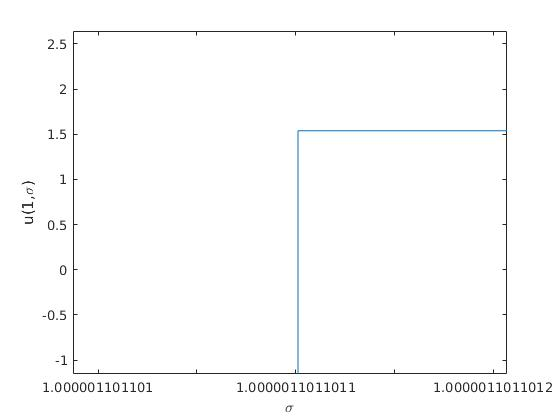
\includegraphics[width=\textwidth]{../Figures/usigma}
    \caption{Solution to the IVP at the last point of the interval for a series of $\sigma$ values close to the optima with $\epsilon = 0.01$}
    \label{fig:usigma}
\end{figure}




Even though, figure shows that \ref{fig:ivpconvergence} for large values of $\epsilon$ Newton's method presents quadratic rate of convergence, the differential equation needed to be solved in every iteration is now larger and hence it takes longer to solve. The secant method is a variation to the Newton's algorithm where the derivative is approximated by finite difference and thus, the algorithm becomes more efficient (table \ref{tab:ipv}). The code for all three algorithms is collected in the appendix.

\subsection{Sensitivities}

In order to find an approximation to the partial derivative of the solution with respect to $\sigma$ we can either solve equation \ref{eq:ivp2} or apply the finite difference method. In both cases we see that for small values of $\epsilon$ the solution becomes very sensible to small variations of $\sigma$. That is the reason why neither Newton's method nor the secant algorithm are able to converge even for initial guesses close to the true solution. The  A way around would be to include an extra parameter that controls the step size every time $\sigma$ is updated.
